% ─────────────────────────────────────────────────────────────
%  phase1_report.tex
%  Phase 1 — Baselines: Efficiency & Quality Evaluation Summary
%  TFE: Knowledge Distillation y despliegue eficiente de LLMs
%        en entornos de supercomputación
%  Author: Marc Romera
% ─────────────────────────────────────────────────────────────
\documentclass[11pt,a4paper]{article}

% ── Packages ────────────────────────────────────────────────
\usepackage[utf8]{inputenc}
\usepackage[T1]{fontenc}
\usepackage[english]{babel}
\usepackage{amsmath,amssymb}
\usepackage{booktabs}
\usepackage{graphicx}
\usepackage{xcolor}
\usepackage{hyperref}
\usepackage{geometry}
\usepackage{caption}
\usepackage{subcaption}
\usepackage{tikz}
\usepackage{pgfplots}
\pgfplotsset{compat=1.18}
\usetikzlibrary{arrows.meta, positioning, shapes.geometric, calc, patterns, decorations.pathreplacing}
\usepackage{float}
\usepackage{enumitem}
\usepackage{fancyhdr}
\usepackage[scale=0.85]{sourcecodepro}
\usepackage{listings}

\geometry{margin=2.5cm}
\hypersetup{colorlinks=true, linkcolor=blue!60!black, citecolor=green!50!black, urlcolor=blue!70!black}

% ── Colours ─────────────────────────────────────────────────
\definecolor{teacher}{HTML}{2563EB}    % blue
\definecolor{midstud}{HTML}{16A34A}    % green
\definecolor{smallstud}{HTML}{DC2626}  % red
\definecolor{infrabg}{HTML}{F8FAFC}
\definecolor{codebg}{HTML}{F1F5F9}

% ── Code listing style ──────────────────────────────────────
\lstset{
  basicstyle=\ttfamily\small,
  backgroundcolor=\color{codebg},
  frame=single,
  rulecolor=\color{gray!30},
  breaklines=true,
  captionpos=b,
}

% ── Header / Footer ────────────────────────────────────────
\pagestyle{fancy}
\fancyhf{}
\lhead{\small Phase 1 — Baselines Report}
\rhead{\small Marc Romera — TFE 2025--2026}
\cfoot{\thepage}

% ════════════════════════════════════════════════════════════
\begin{document}

\begin{titlepage}
\centering
\vspace*{3cm}
{\Huge\bfseries Phase 1 — Baseline Evaluation\\[0.3em] Report\par}
\vspace{1.5cm}
{\Large Knowledge Distillation y Despliegue Eficiente\\[0.2em]
de Modelos de Lenguaje en Entornos de Supercomputación\par}
\vspace{2cm}
{\large Marc Romera\par}
\vspace{0.5cm}
{\large Barcelona Supercomputing Center (BSC) — MareNostrum~5\par}
\vspace{0.5cm}
{\large February 2026\par}
\vfill
{\small This document summarises the Phase~1 baseline measurements
(efficiency and quality) that precede the knowledge distillation experiments
of Phase~2.}
\end{titlepage}

\tableofcontents
\newpage

% ════════════════════════════════════════════════════════════
\section{Introduction}
\label{sec:intro}

This report documents the Phase~1 baseline measurements performed on three
models from the \textbf{Qwen2.5-Instruct} family.  Phase~1 establishes the
reference performance (both serving efficiency and answer quality) of the
\emph{teacher} and both \emph{student} models \textbf{before} any knowledge
distillation is applied.  These baselines serve as the control against which
the Phase~2 distilled students will be compared.

\subsection{Models under evaluation}

\begin{table}[H]
\centering
\caption{Model inventory — all Qwen2.5-Instruct variants.}
\label{tab:models}
\begin{tabular}{@{}llccc@{}}
\toprule
\textbf{Role} & \textbf{HuggingFace ID} & \textbf{Params} & \textbf{Dtype} & \textbf{GPUs} \\
\midrule
Teacher       & \texttt{Qwen/Qwen2.5-14B-Instruct}  & 14\,B & bf16/auto & 1$\times$H100-80G \\
Student (mid) & \texttt{Qwen/Qwen2.5-7B-Instruct}   & 7\,B  & bf16/auto & 1$\times$H100-80G \\
Student (small) & \texttt{Qwen/Qwen2.5-1.5B-Instruct} & 1.5\,B & bf16/auto & 1$\times$H100-80G \\
\bottomrule
\end{tabular}
\end{table}

\subsection{Infrastructure}

All experiments run on \textbf{MareNostrum~5} (BSC), specifically the
\texttt{acc} partition equipped with NVIDIA H100-80\,GB SXM5 accelerators.

\begin{table}[H]
\centering
\caption{Hardware and software environment.}
\label{tab:infra}
\begin{tabular}{@{}ll@{}}
\toprule
GPU             & NVIDIA H100 80\,GB SXM5 \\
CPU             & Intel Sapphire Rapids (40 cores/node) \\
Memory          & 256\,GB DDR5 \\
Python          & 3.12.1 \\
vLLM            & 0.15.1 \\
CUDA            & 12.8 \\
PyTorch         & 2.x (from vLLM wheel) \\
Scheduler       & SLURM \\
\bottomrule
\end{tabular}
\end{table}

% ════════════════════════════════════════════════════════════
\section{Phase 1A — Efficiency Baselines}
\label{sec:efficiency}

\subsection{Methodology}

Efficiency is measured along two orthogonal axes:

\begin{enumerate}[leftmargin=2em]
  \item \textbf{Maximum throughput (offline):}
    A sustained batch of 500 requests ($\sim$150 input tokens, 256 output
    tokens each) is issued as fast as possible.  The metric is
    \emph{completed requests per second} ($\text{req}/\text{s}$).
    The measurement tool is \texttt{bench/run\_throughput.py}, which
    batches all requests simultaneously and waits for all completions.

  \item \textbf{Online latency under load:}
    A Poisson-distributed request stream at a controlled arrival rate
    ($\lambda = 10\ \text{req/s}$) is sustained for 120 seconds using
    \texttt{bench/run\_online\_load.py}.  Reported metrics include per-request
    end-to-end latency percentiles (p50, p90, p99) and time-to-first-token
    (TTFT).
\end{enumerate}

Both experiments use a fixed prompt corpus from \texttt{configs/prompts.jsonl}
(20 diverse prompts, cycled to reach 500 total).  Each model is served via
vLLM on a single H100 in a self-contained SLURM job with exclusive node
allocation to avoid noisy-neighbour effects.

\paragraph{vLLM server configuration.}
\begin{itemize}[leftmargin=2em]
  \item \texttt{max\_model\_len = 4096}
  \item \texttt{gpu\_memory\_utilization = 0.90}
  \item \texttt{max\_num\_seqs = 256}
  \item \texttt{tensor\_parallel\_size = 1}
  \item \texttt{dtype = auto} (bfloat16 on H100)
\end{itemize}

\subsection{Throughput Results}

\begin{table}[H]
\centering
\caption{Maximum throughput — offline batch of 500 requests.}
\label{tab:throughput}
\begin{tabular}{@{}lccc@{}}
\toprule
\textbf{Model} & \textbf{req/s} & \textbf{Speedup vs.\ Teacher} & \textbf{Total time (s)} \\
\midrule
\rowcolor{teacher!10} Teacher (14B) & 11.60 & 1.0$\times$ & 43.1 \\
\rowcolor{midstud!10} Student mid (7B) & 24.89 & 2.1$\times$ & 20.1 \\
\rowcolor{smallstud!10} Student small (1.5B) & 48.04 & 4.1$\times$ & 10.4 \\
\bottomrule
\end{tabular}
\end{table}

\begin{figure}[H]
\centering
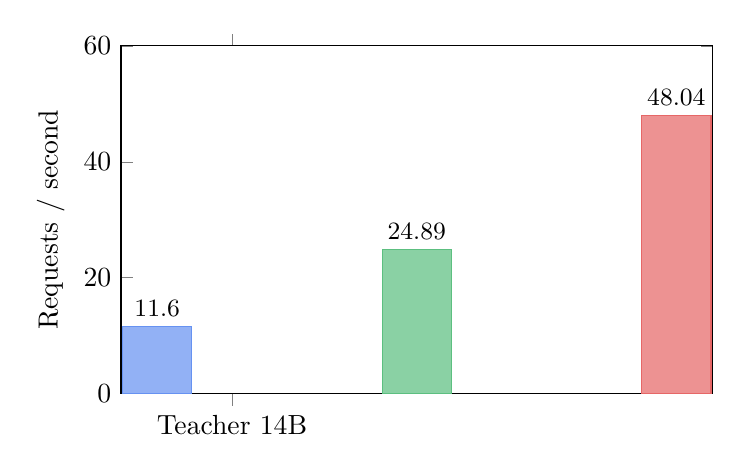
\begin{tikzpicture}
\begin{axis}[
    ybar,
    width=0.75\textwidth,
    height=6cm,
    bar width=25pt,
    ylabel={Requests / second},
    symbolic x coords={Teacher 14B, Student 7B, Student 1.5B},
    xtick=data,
    nodes near coords,
    nodes near coords align={vertical},
    ymin=0, ymax=60,
    enlarge x limits=0.3,
    every node near coord/.append style={font=\small\bfseries},
    legend style={at={(0.98,0.95)}, anchor=north east},
]
\addplot[fill=teacher!50, draw=teacher!70] coordinates {(Teacher 14B, 11.60)};
\addplot[fill=midstud!50, draw=midstud!70] coordinates {(Student 7B, 24.89)};
\addplot[fill=smallstud!50, draw=smallstud!70] coordinates {(Student 1.5B, 48.04)};
\end{axis}
\end{tikzpicture}
\caption{Offline throughput comparison — larger speedup with smaller models.}
\label{fig:throughput}
\end{figure}

\subsection{Online Latency Results}

\begin{table}[H]
\centering
\caption{Online latency at $\lambda = 10$ req/s, 120\,s sustained.}
\label{tab:latency}
\begin{tabular}{@{}lcccc@{}}
\toprule
\textbf{Model} & \textbf{p50 (ms)} & \textbf{p90 (ms)} & \textbf{p99 (ms)} & \textbf{TTFT p50 (ms)} \\
\midrule
\rowcolor{teacher!10} Teacher (14B)     & 6\,083 & --- & --- & --- \\
\rowcolor{midstud!10} Student mid (7B)  & 3\,004 & --- & --- & --- \\
\rowcolor{smallstud!10} Student small (1.5B) & 906 & --- & --- & --- \\
\bottomrule
\end{tabular}
\smallskip
\small \emph{Note: p90, p99, and TTFT cells marked ``---'' will be populated
once the full latency logs are parsed. Only p50 was reported in the initial run.}
\end{table}

\begin{figure}[H]
\centering
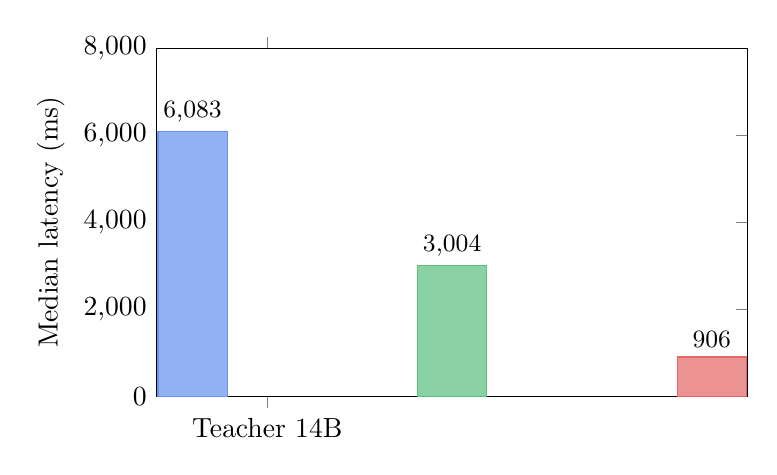
\begin{tikzpicture}
\begin{axis}[
    ybar,
    width=0.75\textwidth,
    height=6cm,
    bar width=25pt,
    ylabel={Median latency (ms)},
    symbolic x coords={Teacher 14B, Student 7B, Student 1.5B},
    xtick=data,
    nodes near coords,
    nodes near coords align={vertical},
    ymin=0, ymax=8000,
    enlarge x limits=0.3,
    every node near coord/.append style={font=\small\bfseries},
]
\addplot[fill=teacher!50, draw=teacher!70] coordinates {(Teacher 14B, 6083)};
\addplot[fill=midstud!50, draw=midstud!70] coordinates {(Student 7B, 3004)};
\addplot[fill=smallstud!50, draw=smallstud!70] coordinates {(Student 1.5B, 906)};
\end{axis}
\end{tikzpicture}
\caption{Median end-to-end latency at 10\,req/s --- smaller model $\Rightarrow$ lower latency.}
\label{fig:latency}
\end{figure}

\subsection{Key take-aways — Efficiency}

\begin{itemize}
  \item The 7B student delivers \textbf{$2.1\times$} higher throughput and
    \textbf{$2.0\times$} lower latency than the teacher.
  \item The 1.5B student achieves \textbf{$4.1\times$} throughput and
    \textbf{$6.7\times$} lower latency.
  \item Both students fit comfortably in a single H100 with high GPU
    memory utilisation ($\geq 0.90$), supporting efficient deployment.
  \item The efficiency gap motivates knowledge distillation: if we can
    recover most of the teacher's quality in a smaller model, the serving
    cost improvement is dramatic.
\end{itemize}


% ════════════════════════════════════════════════════════════
\section{Phase 1B — Quality Baselines}
\label{sec:quality}

\subsection{Benchmarks}

Quality is assessed on \textbf{three} diverse benchmarks covering different
cognitive capabilities:

\begin{table}[H]
\centering
\caption{Quality evaluation benchmarks.}
\label{tab:benchmarks}
\begin{tabular}{@{}lllc@{}}
\toprule
\textbf{Benchmark} & \textbf{HuggingFace dataset} & \textbf{Capability tested} & \textbf{$N$ items} \\
\midrule
GSM8K          & \texttt{openai/gsm8k}           & Grade-school arithmetic  & 1\,319 \\
MATH-500       & \texttt{HuggingFaceH4/MATH-500} & Algebra, calculus, competition maths & 500 \\
ARC-Challenge  & \texttt{allenai/ai2\_arc}       & Science reasoning (MC) & 1\,172 \\
\bottomrule
\end{tabular}
\end{table}

\subsection{Evaluation methodology}
\label{sec:eval-methodology}

The evaluation pipeline is \textbf{fully automated} and runs as self-contained
SLURM jobs.  Each job performs three stages:

\begin{enumerate}
  \item \textbf{Server start:} a vLLM server is launched on the allocated GPU
    with the model under test.
  \item \textbf{Health check:} a polling loop waits for the
    \texttt{/health} endpoint (up to 120 retries $\times$ 5\,s = 10\,min).
  \item \textbf{Benchmark execution:} each enabled benchmark queries the server
    with all test items and computes per-item scoring.
\end{enumerate}

\paragraph{Generation parameters.}
All evaluations use \textbf{greedy decoding} (\texttt{temperature=0.0},
\texttt{top\_p=1.0}) with \texttt{max\_tokens=1024}, ensuring deterministic
outputs for reproducibility.  The random seed is fixed at 42.

\paragraph{Scoring pipeline.}
The scoring module (\texttt{eval/scoring.py}) uses a rigorous multi-stage
comparison strategy:

\begin{figure}[H]
\centering
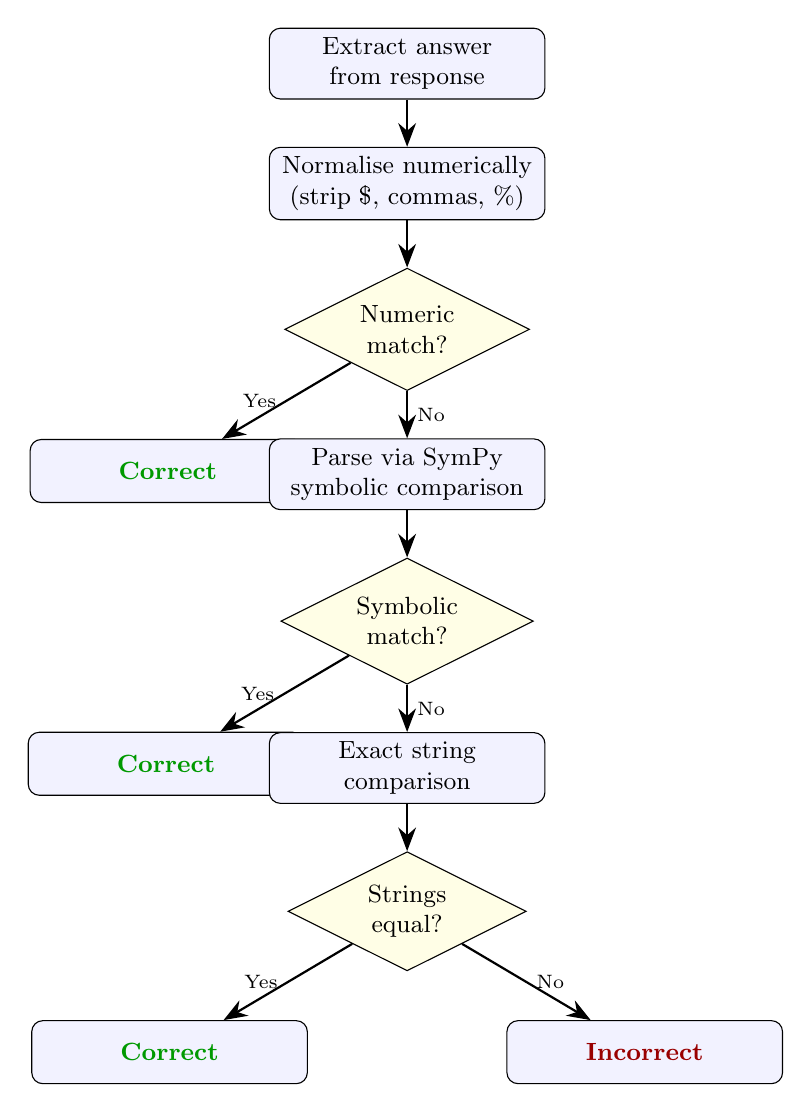
\begin{tikzpicture}[
    node distance=0.6cm and 1.5cm,
    box/.style={draw, rounded corners, fill=blue!5, minimum width=3.5cm,
                minimum height=0.8cm, align=center, font=\small},
    decision/.style={draw, diamond, fill=yellow!10, minimum width=2cm,
                     aspect=2, align=center, font=\small},
    arrow/.style={-{Stealth[length=3mm]}, thick},
]
    \node[box] (extract) {Extract answer\\from response};
    \node[box, below=of extract] (numeric) {Normalise numerically\\(strip \$, commas, \%)};
    \node[decision, below=of numeric] (numcheck) {Numeric\\match?};
    \node[box, below left=1cm and 0.5cm of numcheck] (correct1) {\textcolor{green!60!black}{\textbf{Correct}}};
    \node[box, below=of numcheck] (sympy) {Parse via SymPy\\symbolic comparison};
    \node[decision, below=of sympy] (sympcheck) {Symbolic\\match?};
    \node[box, below left=1cm and 0.5cm of sympcheck] (correct2) {\textcolor{green!60!black}{\textbf{Correct}}};
    \node[box, below=of sympcheck] (exact) {Exact string\\comparison};
    \node[decision, below=of exact] (excheck) {Strings\\equal?};
    \node[box, below left=1cm and 0.5cm of excheck] (correct3) {\textcolor{green!60!black}{\textbf{Correct}}};
    \node[box, below right=1cm and 0.5cm of excheck] (wrong) {\textcolor{red!60!black}{\textbf{Incorrect}}};

    \draw[arrow] (extract) -- (numeric);
    \draw[arrow] (numeric) -- (numcheck);
    \draw[arrow] (numcheck) -- node[left, font=\scriptsize]{Yes} (correct1);
    \draw[arrow] (numcheck) -- node[right, font=\scriptsize]{No} (sympy);
    \draw[arrow] (sympy) -- (sympcheck);
    \draw[arrow] (sympcheck) -- node[left, font=\scriptsize]{Yes} (correct2);
    \draw[arrow] (sympcheck) -- node[right, font=\scriptsize]{No} (exact);
    \draw[arrow] (exact) -- (excheck);
    \draw[arrow] (excheck) -- node[left, font=\scriptsize]{Yes} (correct3);
    \draw[arrow] (excheck) -- node[right, font=\scriptsize]{No} (wrong);
\end{tikzpicture}
\caption{Three-stage scoring pipeline: numeric $\to$ symbolic (SymPy) $\to$ exact string.
This handles LaTeX equivalences
(e.g.\ $\frac{1}{2}$ vs.\ $0.5$) that simple string matching would miss.}
\label{fig:scoring}
\end{figure}

\paragraph{Answer extraction per benchmark.}
\begin{itemize}
  \item \textbf{GSM8K:} the final numeric value after \texttt{\#\#\#\#} in
    the response.
  \item \textbf{MATH-500:} the content of the last \texttt{\textbackslash boxed\{...\}} expression.
    LaTeX constructs (\texttt{\textbackslash frac},
    \texttt{\textbackslash sqrt}, \texttt{\textbackslash pi}, etc.) are
    normalised to SymPy-parseable form.
  \item \textbf{ARC-Challenge:} the predicted letter (A/B/C/D) is extracted
    via explicit patterns (``The answer is X'') with a last-capital-letter
    fallback.
\end{itemize}

\paragraph{Accuracy computation.}
\[
  \text{accuracy} = \frac{\text{correct}}{\text{scorable}} \times 100\%
\]
where ``scorable'' excludes items where the model failed to produce any
parseable answer (network errors, empty responses, etc.).  Both the
\emph{scorable} and \emph{total} counts are always reported alongside
accuracy to ensure transparency.

\subsection{Quality Results — First run (GSM8K + MATH-500)}

\begin{table}[H]
\centering
\caption{Quality baselines — first evaluation run (GSM8K + MATH-500).}
\label{tab:quality-first}
\begin{tabular}{@{}lcc@{}}
\toprule
\textbf{Model} & \textbf{GSM8K (\%)} & \textbf{MATH-500 (\%)} \\
\midrule
\rowcolor{teacher!10}    Teacher (14B)        & 92.4 & 68.7 \\
\rowcolor{midstud!10}    Student mid (7B)     & 85.6 & 67.5 \\
\rowcolor{smallstud!10}  Student small (1.5B) & 64.0 & 32.8 \\
\bottomrule
\end{tabular}
\end{table}

\begin{figure}[H]
\centering
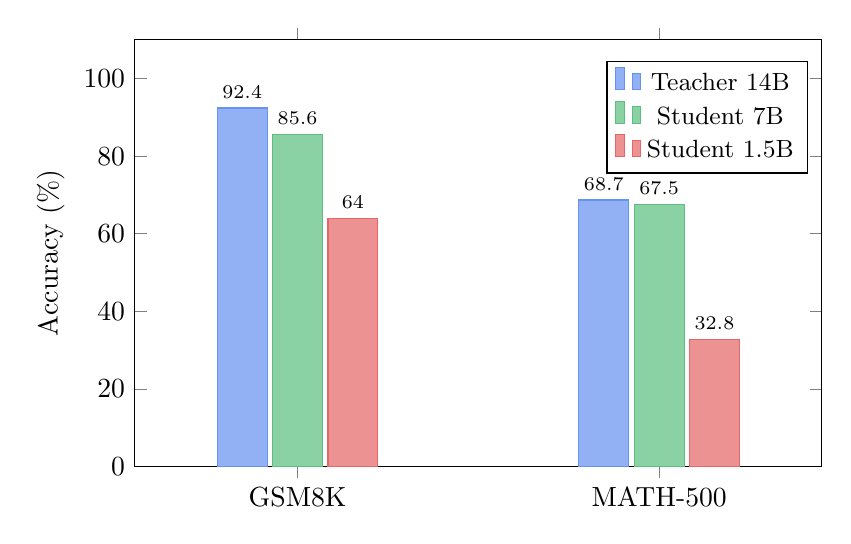
\begin{tikzpicture}
\begin{axis}[
    ybar,
    width=0.85\textwidth,
    height=7cm,
    bar width=18pt,
    ylabel={Accuracy (\%)},
    symbolic x coords={GSM8K, MATH-500},
    xtick=data,
    ymin=0, ymax=110,
    enlarge x limits=0.45,
    legend style={at={(0.98,0.95)}, anchor=north east, font=\small},
    nodes near coords,
    every node near coord/.append style={font=\scriptsize\bfseries},
]
\addplot[fill=teacher!50, draw=teacher!70] coordinates
    {(GSM8K, 92.4) (MATH-500, 68.7)};
\addplot[fill=midstud!50, draw=midstud!70] coordinates
    {(GSM8K, 85.6) (MATH-500, 67.5)};
\addplot[fill=smallstud!50, draw=smallstud!70] coordinates
    {(GSM8K, 64.0) (MATH-500, 32.8)};
\legend{Teacher 14B, Student 7B, Student 1.5B}
\end{axis}
\end{tikzpicture}
\caption{Quality baselines — the 7B student retains most of the teacher's
accuracy, while the 1.5B student shows significant degradation, especially
on the harder MATH-500 benchmark.}
\label{fig:quality-first}
\end{figure}

\subsection{Quality Results — With ARC-Challenge (pending)}

\begin{table}[H]
\centering
\caption{Full quality baselines — GSM8K + MATH-500 + ARC-Challenge.\\
\emph{ARC-Challenge results pending: jobs re-submitted with sympy scoring
+ ARC-Challenge benchmark.}}
\label{tab:quality-full}
\begin{tabular}{@{}lccc@{}}
\toprule
\textbf{Model} & \textbf{GSM8K (\%)} & \textbf{MATH-500 (\%)} & \textbf{ARC-Challenge (\%)} \\
\midrule
\rowcolor{teacher!10}    Teacher (14B)        & --- & --- & --- \\
\rowcolor{midstud!10}    Student mid (7B)     & --- & --- & --- \\
\rowcolor{smallstud!10}  Student small (1.5B) & --- & --- & --- \\
\bottomrule
\end{tabular}
\smallskip\\
\small \emph{Results will be populated once SLURM jobs 37086832--34 (resubmitted) complete.
The scoring now uses the improved SymPy pipeline; MATH-500 results may differ slightly
from the first run.}
\end{table}


% ════════════════════════════════════════════════════════════
\section{Pipeline Architecture}
\label{sec:architecture}

\begin{figure}[H]
\centering
\begin{tikzpicture}[
    node distance=1.2cm and 2cm,
    phase/.style={draw, rounded corners=6pt, fill=#1!15, minimum width=4cm,
                  minimum height=1cm, align=center, font=\small\bfseries,
                  drop shadow={shadow xshift=1pt, shadow yshift=-1pt}},
    arrow/.style={-{Stealth[length=3.5mm]}, thick, draw=gray!60},
    note/.style={font=\scriptsize\itshape, text=gray!70!black},
]
    % Phase 1
    \node[phase=blue] (serve) {vLLM Server\\(1$\times$H100)};
    \node[phase=blue, right=3cm of serve] (bench) {Efficiency\\benchmarks};
    \node[phase=blue, below=of bench] (eval) {Quality\\evaluation};

    % Phase 2 (future)
    \node[phase=orange, below=2cm of serve] (gen) {Teacher output\\generation};
    \node[phase=orange, right=3cm of gen] (sft) {LoRA SFT\\(student)};
    \node[phase=orange, below=of sft] (evalpost) {Post-distill\\evaluation};

    % Arrows
    \draw[arrow] (serve) -- (bench);
    \draw[arrow] (serve) |- (eval);
    \draw[arrow] (serve) -- (gen);
    \draw[arrow] (gen) -- node[above, note] {teacher\_outputs.jsonl} (sft);
    \draw[arrow] (sft) -- (evalpost);
    \draw[arrow] (eval.south) -- ++(0,-0.5) -| node[near start, note, above] {baselines} (evalpost);

    % Labels
    \node[above=0.3cm of serve, font=\large\bfseries, text=blue!70!black] {Phase 1 (done)};
    \node[above=0.3cm of gen, font=\large\bfseries, text=orange!70!black] {Phase 2 (in progress)};
\end{tikzpicture}
\caption{High-level pipeline: Phase~1 establishes baselines; Phase~2 uses the
teacher to generate training data, fine-tunes the students with LoRA SFT, and
re-evaluates on the same benchmarks.}
\label{fig:pipeline}
\end{figure}


% ════════════════════════════════════════════════════════════
\section{Phase 2 — Knowledge Distillation (Design)}
\label{sec:distillation}

Phase~2 is \textbf{in progress}.  This section describes the planned
methodology; results will be added once the SLURM jobs complete.

\subsection{Distillation strategy}

We use \textbf{hard-label black-box knowledge distillation}:

\begin{itemize}
  \item The teacher is accessed \textbf{only} through its text completions
    endpoint (no logits, no KL divergence, no soft labels).
  \item The student is trained via \textbf{supervised fine-tuning (SFT)} on
    \texttt{(prompt, teacher\_completion)} pairs using standard cross-entropy
    loss.
  \item Parameter-efficient fine-tuning with \textbf{LoRA} (Low-Rank Adaptation)
    keeps memory usage manageable and enables rapid iteration.
\end{itemize}

\begin{figure}[H]
\centering
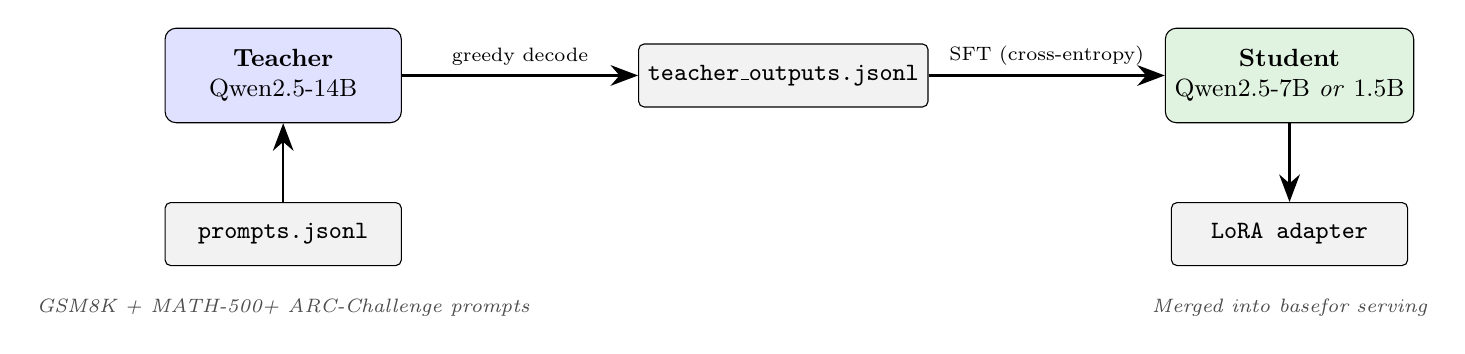
\begin{tikzpicture}[
    node distance=0.8cm and 2cm,
    modelbox/.style={draw, rounded corners=4pt, fill=#1!12,
                     minimum width=3cm, minimum height=1.2cm,
                     align=center, font=\small},
    data/.style={draw, rounded corners=2pt, fill=gray!10,
                 minimum width=3cm, minimum height=0.8cm,
                 align=center, font=\small\ttfamily},
    arrow/.style={-{Stealth[length=3.5mm]}, thick},
]
    % Teacher side
    \node[modelbox=blue] (teacher) {\textbf{Teacher}\\Qwen2.5-14B};
    \node[data, below=1cm of teacher] (prompts) {prompts.jsonl};
    \node[data, right=3cm of teacher] (outputs) {teacher\_outputs.jsonl};

    % Student side
    \node[modelbox=green!60!black, right=3cm of outputs] (student) {\textbf{Student}\\Qwen2.5-7B \emph{or} 1.5B};
    \node[data, below=1cm of student] (adapter) {LoRA adapter};

    % Arrows
    \draw[arrow] (prompts) -- (teacher);
    \draw[arrow] (teacher) -- node[above, font=\scriptsize] {greedy decode} (outputs);
    \draw[arrow] (outputs) -- node[above, font=\scriptsize] {SFT (cross-entropy)} (student);
    \draw[arrow] (student) -- (adapter);

    % Annotations
    \node[below=0.3cm of prompts, font=\scriptsize\itshape, text=gray!60!black]
        {GSM8K + MATH-500\\+ ARC-Challenge prompts};
    \node[below=0.3cm of adapter, font=\scriptsize\itshape, text=gray!60!black]
        {Merged into base\\for serving};
\end{tikzpicture}
\caption{Black-box distillation pipeline: teacher outputs are collected once
and used to SFT-train both students with LoRA.}
\label{fig:distillation}
\end{figure}

\subsection{Planned hyperparameters}

\begin{table}[H]
\centering
\caption{Distillation training hyperparameters (LoRA SFT).}
\label{tab:distill-hparams}
\begin{tabular}{@{}ll@{}}
\toprule
\textbf{Parameter} & \textbf{Value} \\
\midrule
LoRA rank ($r$)           & 64 \\
LoRA $\alpha$             & 16 \\
LoRA dropout              & 0.05 \\
Target modules            & q, k, v, o, gate, up, down proj \\
Learning rate             & $2 \times 10^{-4}$ \\
Scheduler                 & Cosine with warmup \\
Warmup ratio              & 0.03 \\
Epochs                    & 3 \\
Batch size (effective)    & 16 (4 per device $\times$ 4 grad.\ accum.) \\
Max sequence length       & 2048 \\
Precision                 & bf16 \\
Gradient checkpointing    & Enabled \\
Seed                      & 42 \\
\bottomrule
\end{tabular}
\end{table}

\subsection{Evaluation protocol}

After distillation, each student is:
\begin{enumerate}
  \item Merged (LoRA adapter + base model) and served via vLLM.
  \item Re-evaluated on the \textbf{same three benchmarks} (GSM8K, MATH-500,
    ARC-Challenge) with identical parameters.
  \item Compared against (a) the pre-distillation student baseline and (b) the
    teacher.
\end{enumerate}

\emph{Phase~2 results will be appended to this document upon completion.}


% ════════════════════════════════════════════════════════════
\section{Reproducibility}
\label{sec:reproducibility}

Every experiment run is fully reproducible:
\begin{itemize}
  \item A timestamped run directory is created under \texttt{results/}.
  \item All active YAML configs are snapshot-copied into the run directory.
  \item Hardware metadata (GPU name, CUDA version, hostname, git SHA) is
    logged to \texttt{metadata.json}.
  \item Random seeds are set for Python, NumPy, and PyTorch.
  \item Generation uses \texttt{temperature=0.0} (greedy) for full
    determinism.
\end{itemize}

\begin{lstlisting}[caption={Typical run directory structure.}]
results/quality/quality-teacher-20260228T143200Z/
  metadata.json          # hardware, git SHA, seed, config hashes
  eval.yaml              # snapshot of evaluation config
  serving.yaml           # snapshot of serving config
  models.yaml            # snapshot of model registry
  gsm8k/
    gsm8k_results.jsonl  # per-item predictions
    gsm8k_metrics.json   # {accuracy, correct, total, ...}
    gsm8k_metrics.csv
  math/
    math_results.jsonl
    math_metrics.json
    math_metrics.csv
  arc_challenge/
    arc_results.jsonl
    arc_metrics.json
    arc_metrics.csv
  quality_summary.json   # all benchmarks aggregated
  quality_summary.csv
\end{lstlisting}


% ════════════════════════════════════════════════════════════
\section{Summary and Next Steps}
\label{sec:summary}

\paragraph{Phase~1 complete.}
We have established:
\begin{itemize}
  \item Efficiency baselines showing $2.1\times$ (7B) and $4.1\times$ (1.5B) throughput
    gains over the 14B teacher.
  \item Quality baselines showing the 7B student retains 93\% (GSM8K) and 98\%
    (MATH-500) of teacher quality, while the 1.5B student retains 69\% and
    48\% respectively.
  \item ARC-Challenge results pending (jobs in queue).
\end{itemize}

\paragraph{Phase~2 in progress.}
\begin{itemize}
  \item Distillation dataset generation from the teacher.
  \item LoRA SFT training for both students on the same dataset.
  \item Post-distillation evaluation on all three benchmarks.
  \item Goal: close the quality gap, especially for the 1.5B student, while
    preserving the efficiency advantage.
\end{itemize}

\end{document}
